\documentclass[12pt,a4paper,table]{article}

\usepackage[a4paper,
            tmargin=2cm,
            bmargin=2cm,
            lmargin=2cm,
            rmargin=2cm,
            bindingoffset=0cm]{geometry}

\usepackage{lmodern}
\usepackage[T1]{polski}
\usepackage[utf8]{inputenc}
\usepackage{tocloft}
\usepackage{hyperref}
\usepackage{amsmath}
\usepackage{listings}
\usepackage{graphicx}
\usepackage{subfig}
\usepackage{float}
\usepackage{booktabs}

\hypersetup{
    colorlinks,
    citecolor=black,
    filecolor=black,
    linkcolor=black,
    urlcolor=black
}

\newtheorem{definition}{Def}


\begin{document}
    \title {
        Symulacja Systemów i Modelowanie \\
        Raport 1 \\
        Podstawowy wariant Flocking Algorithm i implementacja w Pythonie

    }

    \author{
        Adam Staniszewski \\
        Dariusz Królicki
    }

    \date{\today}

    \maketitle

    \tableofcontents
    \newpage

    \section{Omówienie zadania do rozwiązania w ramach projektu}
    Celem projektu jest przygotowanie symulacji poruszającego się klucza ptaków. Zadanie okazuje się zaskakująco nieskomplikowane - klucz ptaków można zamodelować za pomocą algorytmu zwanego \textbf{Flocking Alogrithm}.

    Mając klucz ptaków, składający się z osobników charakteryzowanych przez wektory ich przemieszczenia i prędkości, oraz ich pole widzenia. Ptaki, znajdujące się nawzajem w swoich polach widzenia, należą do jednej grupy. Na wszystkie osobniki nakładamy następujące ograniczenia:
    \begin{enumerate}
        \item \textbf{Alignment} - każdy osobnik porusza się w kierunku, będącym uśrednionym kierunkiem osobników w jego polu widzenia;
        \item \textbf{Cohesion} - osobniki w grupie poruszają się wokół swojego środka masy;
        \item \textbf{Separation} - osobniki muszą być od siebie oddalone o pewną odległość;
    \end{enumerate}

    Oprócz ptaków, symulacja posiada również przeszkody, które mają być omijane przez klucz w finalnej wersji projektu.
    
    \section{Implementacja w Pythonie}
    Do implementacji algorytmu został użyty Python, w tym biblioteka PyGame, umożliwiająca bardzo proste tworzenie interfejsów graficznych. Przygotowany podczas pierwszego etapu prac kod składa się z czterech części, umówionych poniżej.
    \subsection{bird.py}
    Klasa \textbf{bird.py} obłusugje zachowanie pojedynczego osobnika w stadzie, w tym:
    \begin{enumerate}
        \item Aktualizowanie pozycji w oparciu o inne ptaki z gtuby (alignment, cohesion i separation);
        \item Aktualizowanie pozycji ptaka w przypadku znalezienia siępoza obszarem symulacji;
        \item Sprawdzanie, czy ptak nie wszedł w kolizję z przeszkodą, i potencjalne usuwanie go;
    \end{enumerate}

    \raggedright
    \vskip
    Konstruktor klasy bird.py:
    \begin{lstlisting}[language=Python]
    def __init__(self, x: int, y: int, size: int, perception_radius: int):
        """
        Constructor
        """
        self.position = pygame.Vector2(x, y)
        self.velocity = pygame.Vector2(random.uniform(-1, 1), 
                                random.uniform(-1, 1))
        self.velocity.scale_to_length(MAX_SPEED)
        self.size: int = size
        self.perception_radius: int = perception_radius
    \end{lstlisting}

    \raggedright
    \newpage
    Aktualizacja pozycji osobnika:
    \begin{lstlisting}[language=Python]
    def update(self, flock: List[Bird], obstacles) -> None:
        """
        Update bird's position using flocking algorithm
        """
        self.position += self.velocity

        self.wrap_edges()

        avg_velocity = pygame.Vector2(0, 0)
        avg_position = pygame.Vector2(0, 0)
        avg_separation = pygame.Vector2(0, 0)
        num_neighbors = 0

        for other in flock:
            if other == self:
                continue

            distance_squared = self.distance_to(other)

            if distance_squared < self.perception_radius ** 2:
                avg_velocity += other.velocity
                avg_position += other.position

                if distance_squared < SEPARATION_DISTANCE ** 2:
                    diff = self.position - other.position
                    diff.scale_to_length(1 / distance_squared)
                    avg_separation += diff

                num_neighbors += 1

        if num_neighbors > 0:
            avg_velocity /= num_neighbors
            avg_position /= num_neighbors
            avg_separation /= num_neighbors

        self.velocity += avg_velocity * 0.02
        self.velocity += avg_position * 0.01
        self.velocity += avg_separation * 0.03

        self.velocity.scale_to_length(MAX_SPEED)

        self.check_collisions(obstacles, flock)
    \end{lstlisting}

    \raggedright
    \newpage
    Przenoszenie osobnika na drugą stronę ekranu, jeśli znajdzie się poza obszarem symulacji:
    \begin{lstlisting}[language=Python]
        def wrap_edges(self) -> None:
            """
            Move the bird to the other side of 
            the screen if it goes off the boundaries
            """
            width, height = pygame.display.get_surface().get_size()
            if self.position.x < 0:
                self.position.x = width
            if self.position.y < 0:
                self.position.y = height
            if self.position.x > width:
                self.position.x = 0
            if self.position.y > height:
                self.position.y = 0
    \end{lstlisting}

    \raggedright

     Sprawdzanie kolizji:
    \begin{lstlisting}[language=Python]
    def check_collisions(self, obstacles, flock: List[Bird]) -> None:
        """
        Check if a bird collided with an obstacle, if so, 
        remove it from the list representing flock
        """
        for obstacle in obstacles:
            dx = self.position[0] - obstacle.position[0]
            dy = self.position[1] - obstacle.position[1]
            distance_squared = dx ** 2 + dy ** 2
            if distance_squared < (self.size + obstacle.radius) ** 2:
                flock.remove(self)
                pygame.event.post(pygame.event.Event(COLLISION_EVENT))
                return
    \end{lstlisting}
    
    \subsection{obstacle.py}
    Klasa \textbf{obstacle.py} przyjmuje w swoim konstruktorze koordynaty, promień oraz obszar, na którym ma się znaleźć. Na tym etapie nie posiada jeszcze żadnych innych funkcji.

    Konstruktor klasy:
    \begin{lstlisting}[language=Python]
        def __init__(self, x, y, radius, screen):
            self.position = (x, y)
            self.screen = screen
            self.radius = radius
    \end{lstlisting}
    \subsection{environment.py}
    Klasa \textbf{environment.py} obsługuje wyświetlanie symulacji, generowanie klucza ptaków oraz przeszkód. Ważniejsze częsci jej kodu:
    \begin{lstlisting}[language=Python]
    def handle_events(self):
        """
        Handle events in the simulation
        """
        for event in pygame.event.get():
            if (event.type == pygame.locals.QUIT
                    or (event.type == pygame.locals.KEYDOWN and 
                        event.key == pygame.locals.K_ESCAPE)):
                self.running = False
            elif event.type == COLLISION_EVENT:
                self.spawn_new_bird(
                    x = random.randint(0, self.screen_options['WIDTH']),
                    y = random.randint(0, self.screen_options['HEIGHT']),
                    size=self.bird_options['SIZE'],
                    perception_radius=self.bird_options['PERCEPTION_RADIUS']
                )

    def start(self):
        self.setup_display()

        for _ in range(self.bird_options['AMOUNT']):
            self.spawn_new_bird(
                x = random.randint(0, self.screen_options['WIDTH']),
                y = random.randint(0, self.screen_options['HEIGHT']),
                size = self.bird_options['SIZE'],
                perception_radius = self.bird_options['PERCEPTION_RADIUS']
            )
        
        for i in range(len(self.obstacle_options['POSITIONS'])):
            self.spawn_new_obstacle(
                x = self.obstacle_options['POSITIONS'][i][0],
                y = self.obstacle_options['POSITIONS'][i][1],
                screen = self.screen
            )
    \end{lstlisting}
    
    \subsection{main.py}
    Klasa \textbf{main.py} przechowuje między innymi liczebność elementów symulacji i wywołuje kolejne metody klasy \textbf{environment.py}

    \subsection{GUI symulacji}
    W przygotowanym GUI (rysunek 1), ptaki reprezentowane są przez białe koła, czerwone okręgi to pola widzenia ptaków, a zielone koła to przeszkody.
    
    \begin{figure}[H]
        \centering
        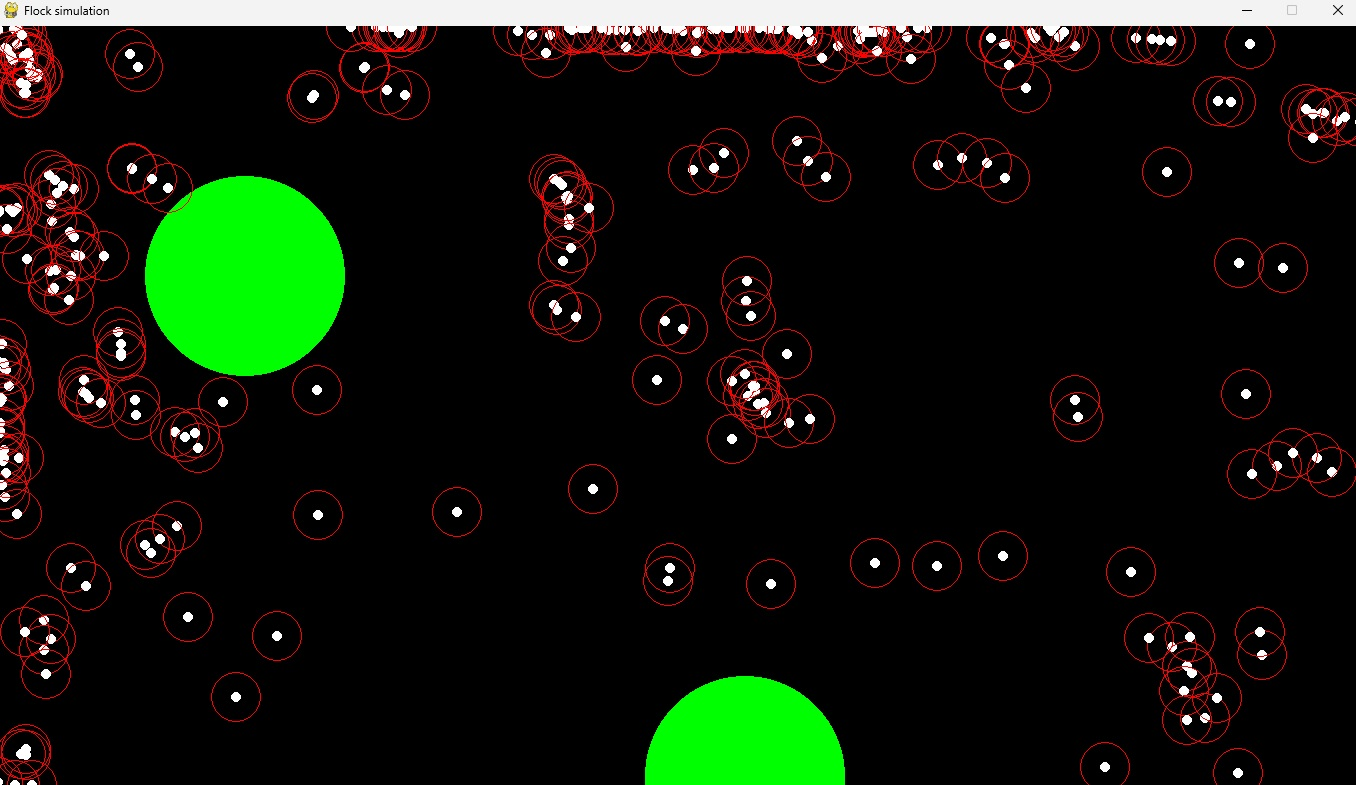
\includegraphics[width=0.8\textwidth]{images/gui1.jpg}
        \caption{Wstęna wersja GUI symulacji}
        \label{fig:example}
    \end{figure}

    \section{Kolejne planowane etapy rozwoju projektu}
    Potencjalne dalsze kroki rozwoju dotyczą optymalizacji symulacji i implementacji modułu uczenia mszynowego.
    \subsection{Optymalizacja symulacji}
    Ze względu na dużą ilość operacji wykonywanych w ramach symulacji, rozważane jest przepisanie jej w języku oferującym lepszą wydajność, na przykład w C++.
    
    \subsection{Algorytm uczący}
    W celu nauczenia osobników omijania pojawiających się przeszkód, można zastosować algorytm uczenia przez wzmocnienie, na przykład Q-Learning.

    \vspace{2em}

    Repozytorium kodu dostępne pod adresem:
    \url{https://github.com/StaniszewskiA/SSIM-Proj}

\end{document}